\documentclass[11pt]{article}
\usepackage{graphicx}
\usepackage{listings}
\usepackage[utf8]{inputenc}
%Gummi|065|=)
\title{\textbf{Machinery Learning  \\ Azure ML}}
\author{
Ana Karen sánchez González A01551014 \\ 
Luis Andrés Juárez Sandoval A01550175}
\date{Mayo 2016}

\begin{document}

\maketitle
\newpage

\section{Introducción}


\textbf{¿Qué es Machine Learning? }\\

Los datos se guardan secretos, especialmente si usted tiene un montón de ellos. Con una gran cantidad de datos acerca de algo, puede examinar los datos de manera inteligente para encontrar patrones. Y esos patrones, que suelen ser demasiado complejos para que usted pueda detectar a sí mismo, se puede decir cómo resolver un problema.\\

Esto es exactamente lo que hace la máquina de aprendizaje: Se analiza grandes cantidades de datos en busca de patrones, a continuación, genera un código que le permite reconocer esos patrones en datos nuevos. Las aplicaciones pueden utilizar este código generado para hacer mejores predicciones. En otras palabras, la máquina de aprendizaje puede ayudar a crear aplicaciones más inteligentes.\\

Por ejemplo, supongamos que desea crear un software que puede determinar, con un alto grado de precisión, si una transacción de tarjeta de crédito es fraudulenta. ¿Cuál es el enfoque correcto para hacer esto? Una opción es obtener unas pocas personas inteligentes juntos en una habitación y pensar en ello, a continuación, escribir código que implementa lo que sea que ocurra. Este es probablemente el método más común para la creación de soluciones de software de hoy en día, y que sin duda puede trabajar.\\

Pero si hay datos disponibles sobre el problema que estamos tratando de resolver, en su lugar puede utilizar esos datos para calcular una solución eficaz. Por ejemplo, supongamos que usted está tratando de encontrar el mejor enfoque para la detección de fraude de tarjetas de crédito, y todo lo que tiene que trabajar con los datos históricos es que se muestran en la figura:\\

\begin{figure}[htp]
\centering
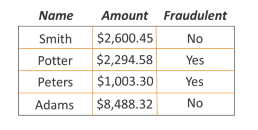
\includegraphics[width=7.5cm]{a.jpg}
\label{fig:lion}
\end{figure}


\newpage

Lo bueno de tener tan pocos datos es que puede ser capaz de encontrar un patrón con sólo mirarlo. Lo malo de tener tan pocos datos es que el patrón que se encuentra es probable que sea errónea. Teniendo en cuenta los datos de la Figura 1, por ejemplo, puede decidir que cualquier persona cuyo nombre comienza con "P" es un estafador, aunque probablemente en otros casos no lo sea.

Si ahora tenemos muchos datos como en la Figura 2:

\begin{figure}[htp]
\centering
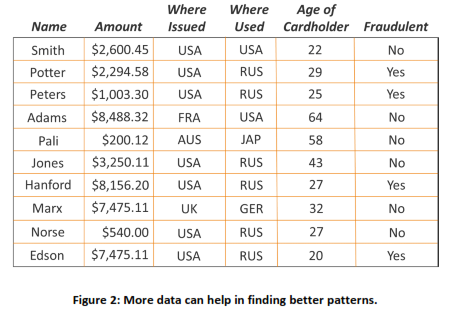
\includegraphics[width=13cm]{b.jpg}
\label{fig:lion}
\end{figure}


La verdad es que el patrón de los datos que apoya es la siguiente: Una transacción es fraudulenta si el titular de la tarjeta es de unos 20 años, la tarjeta fue emitida en los EE.UU. y se utiliza en Rusia, y la cantidad es más de  1,000 Usd Con un poco de tiempo, probablemente habría dado cuenta de esto, ya que los datos que usted tiene que trabajar con no es muy grande.\\

Pero supongamos que tiene no sólo el registro diez para trabajar, como en la figura 2, pero diez millones. Y supongamos que, para cada registro, usted tiene no sólo las seis columnas de datos que se muestran en la Figura 2, pero 60 columnas. Probablemente hay un patrón útil escondido en que los datos para determinar qué transacciones son propensos a ser fraudulenta, pero nunca lo descubrirán por buscar manualmente en la técnica de que hay demasiado de él. En su lugar, usted tiene que utilizar técnicas estadísticas, los enfoques que están diseñados para la búsqueda de patrones en grandes cantidades de datos. Y tendrá que aplicar estas técnicas a los datos mediante su ejecución en un ordenador.\\

Esto es exactamente lo que hace el proceso de aprendizaje de la máquina: Se aplica técnicas estadísticas para grandes cantidades de datos, buscando el mejor patrón para resolver su problema. A continuación, genera una implementación de código que puede reconocer ese patrón. Este código generado se conoce como un modelo, y puede ser llamada por las aplicaciones que necesitan para resolver este problema. Con la detección de fraudes, por ejemplo, la aplicación de llamada debe proporcionar la información correcta acerca de una transacción, tales como la edad, la cantidad, que se emitió la tarjeta, y hacia dónde se está utilizando. El modelo creado a través del aprendizaje de máquina a continuación, devuelve una indicación de si esta operación es probable que sea fraudulenta.\\

Azure Machine Learning (ML azul) es un servicio en la nube que ayuda a las personas que ejecutan el proceso de aprendizaje de la máquina. Como su nombre indica, se ejecuta en Microsoft Azure, una plataforma de nube pública. Debido a esto, Azure ML puede trabajar con grandes cantidades de datos y acceder desde cualquier parte del mundo. Su uso requiere sólo un navegador web y una conexión a Internet.\\


Aun así, la comprensión de lo que hace esta tecnología requiere un análisis más profundo de cómo el aprendizaje de máquina funciona de verdad. La siguiente sección proporciona una visión general del proceso.\\

\newpage
\section{Cómo trabaja Machinery Learning }

El proceso que una organización utiliza Azure ML u otro método, el proceso básico de aprendizaje automático es prácticamente la misma. La figura muestra la forma en que normalmente se ve.


\begin{figure}[htp]
\centering
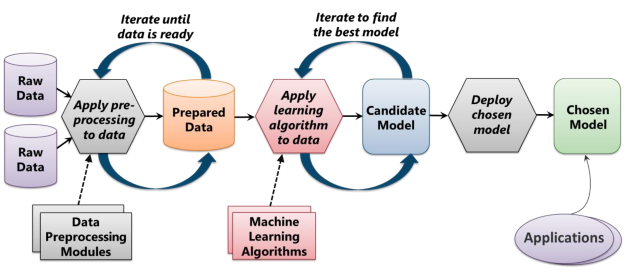
\includegraphics[width=13cm]{c.jpg}
\label{fig:lion}
\end{figure}

Como muestra la figura, la máquina de aprendizaje comienza con datos más se tiene, mejores serán sus resultados son susceptibles de ser. Debido a que vivimos en la gran época de datos, aprendizaje automático se ha convertido en mucho más popular en los últimos años. Tener una gran cantidad de datos para trabajar en muchas áreas diferentes permite las técnicas de aprendizaje de máquina pueden aplicar a un conjunto más amplio de problemas.\\


Dado que el proceso comienza con los datos, la elección de los datos correctos para trabajar es de importancia crítica. Por ejemplo, los datos que debemos usar para detectar el fraude de tarjetas de crédito. Algunas cosas son evidentes, como la edad de un cliente, el país en que se emitió la tarjeta, y el lugar se está utilizando la tarjeta. Sin embargo, otros datos también pueden ser relevantes, tales como la hora del día se utiliza la tarjeta, el tipo de establecimiento que está siendo utilizado en, y tal vez incluso el tiempo en el momento de uso. La determinación de los datos más relevantes para un proyecto de aprendizaje automático es una parte fundamental del proceso, y es un área donde los expertos de dominio por lo general tienen mucho que ofrecer. ¿Quién mejor para decidir cuáles son los indicadores probables de fraude son de hombres de negocios que trabajan en esta área?\\

Sea cual sea su elección de datos, a menudo no está en las condiciones adecuadas para utilizarse directamente. En cambio, los proyectos de aprendizaje automático normalmente procesan los datos brutos con módulos de pre-procesamiento de datos diferentes, como muestra la Figura 3. Con la detección de fraude de tarjetas de crédito, por ejemplo, los datos crudos pueden contener entradas duplicadas para algunos clientes, tal vez con información contradictoria. O los datos crudos pueden contener agujeros, tales como la falta de información acerca de dónde se emitieron o se utilizan algunas tarjetas.\\

El objetivo de pre-procesamiento de datos es crear lo que se llama datos preparados. Pero para llegar hasta aquí por lo general no es simple. Como muestra la Figura 3, que es un proceso iterativo, con varios módulos de pre-procesamiento de datos diferentes aplicados a los datos en bruto. De hecho, la elección de los mejores datos en bruto para empezar, a continuación, la creación de datos preparados a partir de los datos en bruto toma con frecuencia constituyen la mayor parte del tiempo total dedicado a un proyecto de aprendizaje automático.\\

Una vez que un equipo de aprendizaje máquina tiene los datos correctos preparado, se puede pasar a la siguiente etapa: la búsqueda de la mejor manera de resolver el problema que están trabajando, tales como la detección de fraude de tarjetas de crédito. Para ello, el equipo utiliza algoritmos de aprendizaje automático para trabajar con los datos preparados. Estos algoritmos se aplican normalmente un análisis estadístico para los datos. Esto incluye cosas relativamente comunes, como una regresión, junto con enfoques más complejos, incluidos los algoritmos con nombres como de dos clases de árbol de decisión potenciado y selva decisión multi-clase. científico de datos del equipo elige un algoritmo de aprendizaje automático, decide qué se deben usar los aspectos de los datos preparados, a continuación, examina el resultado. El objetivo es determinar qué combinación de algoritmo de aprendizaje automático y datos preparados genera los resultados más útiles. Por ejemplo, si el objetivo es determinar si una transacción de tarjeta de crédito es fraudulenta, el científico de datos escoge las partes de los datos preparados y un algoritmo que se piensa tienen más probabilidades de predecir con precisión este.\\

Como se mencionó anteriormente, cuando un algoritmo de aprendizaje automático se ejecuta en los datos preparados, el resultado se conoce como un modelo. Un modelo es de código que es la aplicación de un algoritmo para el reconocimiento de un patrón, por ejemplo, determinar si una transacción de tarjeta de crédito es fraudulenta. Pero no se confundan: Un algoritmo de aprendizaje automático y el algoritmo implementado por un modelo son cosas diferentes. El algoritmo de aprendizaje automático se ejecuta sobre los datos preparados, y el objetivo es crear un modelo. El algoritmo implementado por el modelo en sí mismo proporciona una solución que resuelve un problema en realidad. Los modelos se acceden por las aplicaciones para responder a preguntas como "¿Es esta transacción fraudulenta?" Algoritmos de aprendizaje automático se utilizan sólo durante el propio proceso de aprendizaje de la máquina.\\

También es importante entender que un modelo típicamente no devuelve un sí o ninguna respuesta. En su lugar, devuelve una probabilidad entre 0 y 1. Decidir qué hacer con esta probabilidad es generalmente una decisión de negocios. Por ejemplo, si un modelo de fraude de tarjetas de crédito devuelve una probabilidad de 0,9, esto dará lugar probablemente a la transacción que se está marcado como fraudulenta, mientras que una probabilidad de 0,1 dejará que la transacción será procesada normalmente. Pero ¿y si el modelo registra una probabilidad de fraude de 0,5? ¿En caso de ser aceptada la transacción, o debería ser bloqueada como fraudulentas? La respuesta a esta pregunta es una decisión de negocios. ¿Es más importante para coger las transacciones fraudulentas, incluso con el riesgo de dar un buen cliente una mala experiencia? ¿O es mejor aceptar un cierto nivel de fraude para evitar que los clientes honestos molestos? Estas son preguntas que los científicos y desarrolladores de datos no se suelen contestar; son temas de negocios.\\

En casi todos los casos, el primer modelo creado candidato no es la mejor. En cambio, el científico de datos intentará muchas combinaciones diferentes de algoritmos de aprendizaje automático y datos preparados, en busca de la que produce el mejor modelo. Cada uno de estos intentos (es decir, cada iteración) puede ser pensado como un experimento, y los proyectos típicos se ejecutará muchos experimentos durante la búsqueda del modelo adecuado, tal como sugiere la figura 3.\\

Una vez que existe un modelo eficaz, hay un paso más: la implementación de ese modelo. Esto permite a las aplicaciones utilizar el algoritmo implementa el modelo. Esta es una parte importante del proceso, sin despliegue, todo el trabajo hecho hasta ahora no sirve para nada. Y si la implementación es demasiado difícil, las personas que crean el modelo no puede ser capaz de desplegar nuevos modelos rápidamente, algo que a menudo se requiere en nuestro mundo que cambia rápidamente.\\

Sin embargo, se desplegó, un modelo implementa un algoritmo de reconocimiento de patrones. Y ¿de dónde ese modelo viene? Fue derivado de los datos. En lugar de poner unas pocas personas inteligentes en una habitación y dejar que ellos inventan una forma de resolver un problema, en lugar de aprendizaje de máquina genera una solución efectiva a partir de datos. Cuando usted tiene un montón de datos para trabajar, esto puede ser un método muy eficaz.\\

\newpage

\section {Azure Machinery Learning}

The machine learning process isn’t especially simple. To make life easier for people doing machine learning, Azure ML provides several different components. Figure 4 shows what those components are and where they fit into the machine learning process.  


\begin{figure}[htp]
\centering
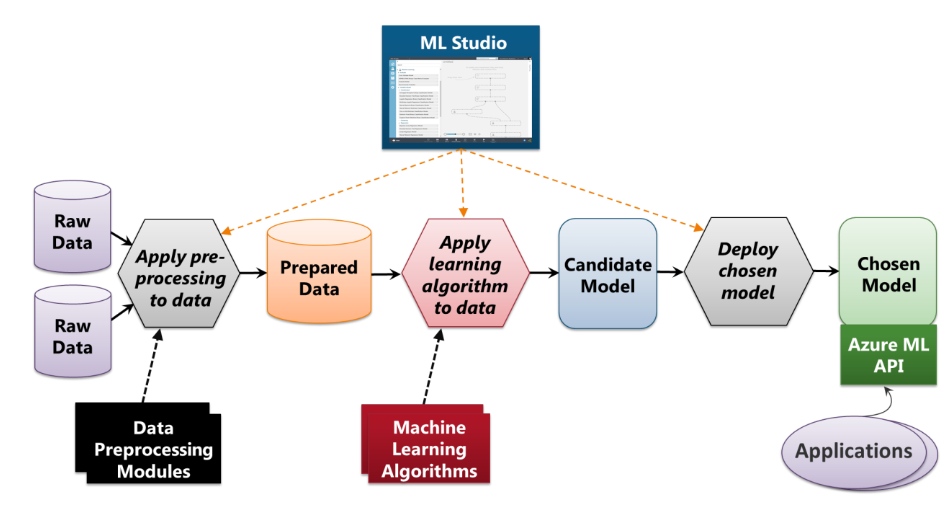
\includegraphics[width=13cm]{d.jpg}
\label{fig:lion}
\end{figure}


ML Studio, a graphical tool that can be used to control the process from beginning to end. Using this tool, people on the machine learning team can apply data preprocessing modules to raw data, run experiments on the prepared data using a machine learning algorithm, and test the resulting model. Once an effective model is found, ML Studio also helps its users deploy that model on Microsoft Azure.\\

\begin{itemize}
  \item A set of data preprocessing modules.
  \item A set of machine learning algorithms.  
  \item An Azure ML API that lets applications access the chosen model once it’s deployed on Azure.
\end{itemize}

All of these are important, and we’ll examine them a bit more closely later. For now, however, it’s worth looking in a little more detail at ML Studio. Figure 5 shows an example of the user interface this tool provides.  

\newpage
\section{Instalación}


Azure se utiliza directamente en la nube es decir no requiere de mucho esfuerzo ya que su interfaz está diseñada para ser utilizada de principio a fin sin utilizar mucho código 

\begin{figure}[htp]
\centering
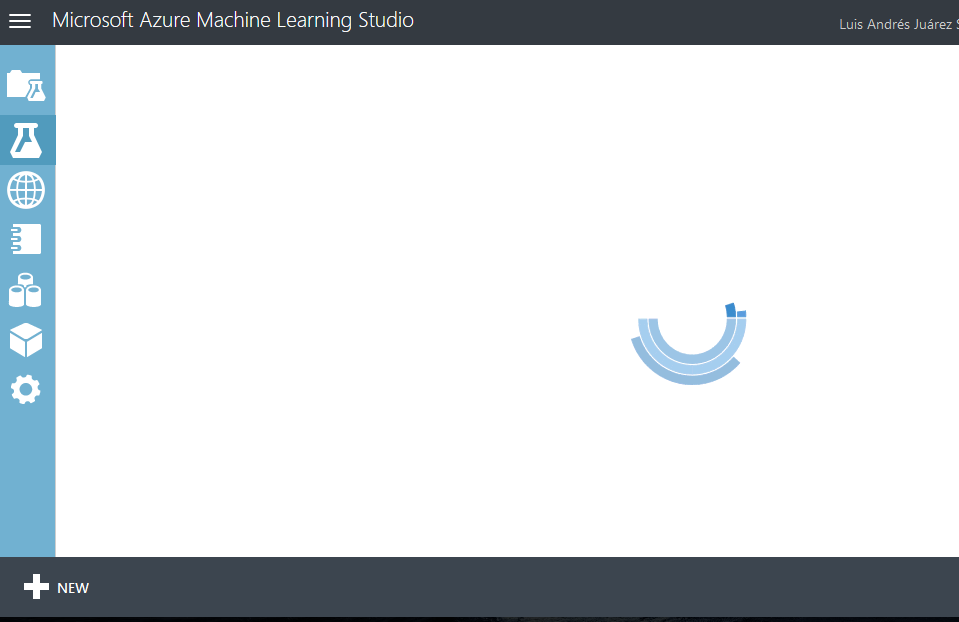
\includegraphics[width=12cm]{e.jpg}
\label{fig:lion}
\end{figure}


\section{Machine Learning Studio: Crea modelos predictivos}

Crear modelos predictivos en Machine Learning Studio, una herramienta basada en navegador, por arrastrar, soltar, y los módulos de conexión. Es decir, desde principio a fin no se requiere de la inserción de código, por lo que cualquier persona puede operar la herramienta si mayor problema y obtener los beneficios que finalmente la herramienta provee 



\begin{figure}[htp]
\centering
\includegraphics[width=13cm]{6.jpg}
\label{fig:lion}
\end{figure}


\section{Configuración}

Para poder utilizar estos servicios de Azure ML es muy sencillo simplemente necesitamos crea una cuenta de Microsoft o en su defecto una cuenta estudiantil con Acceso a Dreamspark para que con ella podamos explotar el máximo de la herramienta, la cual cuenta con un sin fin de métodos como lo son regresión linear, leyes gaussianas y demás. Adicionalmente se puede descargar ciertos complementos, para utilizarlos de manera offline desde su repositorio en GitHub.


\begin{figure}[htp]
\centering
\includegraphics[width=12cm]{8.jpg}
\label{fig:lion}
\end{figure}

\newpage
\section {Laboratorio 1: \\  Cómo predecir si un tiro penal será GOL utilizando Azure ML}

1. Primero debemos ingresar a la Machine Learning de Azure

\begin{figure}[htp]
\centering
\includegraphics[width=12cm]{lab1/0.jpg}
\label{fig:lion}
\end{figure}

\newpage
2. Posteriormente es necesario definir un conjunto de datos en este caso tendremos cuatro columnas con datos aleatorios (Gol, ArqueroAltura, Lugar, Fuerza)
1 representa un gol y -1 un fallo\\

\begin{figure}[htp]
\centering
\includegraphics[width=10cm]{lab1/2.jpg}
\label{fig:lion}
\end{figure}

\newpage
3. También se debe tener otro conjunto de datos más pequeño para utilizarlo de prueba, estos datos son aun más aleatorios con el propósito de abarcar el mayor numero de casos posibles a presentarse.\\ 

\begin{figure}[htp]
\centering
\includegraphics[width=12cm]{lab1/1.jpg}
\label{fig:lion}
\end{figure}

\newpage
4. Este par de conjunto de datos deben ponerse a disposición del proyecto por lo cual los importamos en una extensión csv.\\
\begin{figure}[htp]
\centering
\includegraphics[width=12cm]{lab1/6.jpg}
\label{fig:lion}
\end{figure}

\begin{figure}[htp]
\centering
\includegraphics[width=12cm]{lab1/3.jpg}
\label{fig:lion}
\end{figure}

\begin{figure}[htp]
\centering
\includegraphics[width=12cm]{lab1/4.jpg}
\label{fig:lion}
\end{figure}

\newpage

5. Ahora procedemos a la parte de experimentos y creamos uno nuevo para implementar estos datos.
\begin{figure}[htp]
\centering
\includegraphics[width=12cm]{lab1/5.jpg}
\label{fig:lion}
\end{figure}

\newpage


6. Creamos la red neuronal y su comportamiento, utilizando los conjuntos de datos con sus datasets
\begin{figure}[htp]
\centering
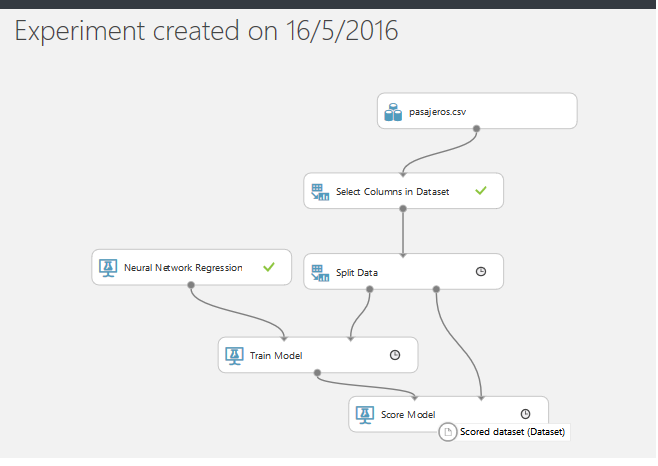
\includegraphics[width=12cm]{lab1/7.jpg}
\label{fig:lion}
\end{figure}




7. Se entrena y prueba el modelo 

\begin{figure}[htp]
\centering
\includegraphics[width=12cm]{lab1/8.jpg}
\label{fig:lion}
\end{figure}

\newpage



8. Procedemos a ver el modelo entrenado, vemos que los datos coinciden y son verídicos a la predicción realizada por la red neuronal.
\begin{figure}[htp]
\centering
\includegraphics[width=12cm]{lab1/9.jpg}
\label{fig:lion}
\end{figure}


9. Dentro de estos datos obtenidos como resultado de la red neuronal podemos observar que las ultimas dos columnas corresponde a los datos en términos clasificatorios y en términos probabilísticos. Es decir que muestran las probabilidades de que ocurra un gol en las condiciones establecidas. 
\begin{figure}[htp]
\centering
\includegraphics[width=12cm]{lab1/8.jpg}
\label{fig:lion}
\end{figure}

\newpage


\section {Laboratorio 2: \\  Predecir la cantidad de pasajeros en el metro usando Azure ML}


Para comenzar el laboratorio iremos al siguiente enlace donde se encuentra el portal de Azure ML 
https://studio.azureml.net\\

\begin{figure}[htp]
\centering
\includegraphics[width=12cm]{2.jpg}
\label{fig:lion}
\end{figure}

Después seleccionaremos la opción new y subiremos una serie de datos de prueba, en la sección Data Set, importando el archivo “pasajeros.csv” \\

\begin{figure}[htp]
\centering
\includegraphics[width=12cm]{3.jpg}
\label{fig:lion}
\end{figure}


Una vez realizada la subida procederemos a crear nuestro experimento desde la opción experiment\\

\begin{figure}[htp]
\centering
\includegraphics[width=12cm]{1.jpg}
\label{fig:lion}
\end{figure}


Obtendremos la siguiente interfaz y agregaremos los módulos tal como se ve en la imagen siguiente\\

\begin{figure}[htp]
\centering
\includegraphics[width=12cm]{4.jpg}
\label{fig:lion}
\end{figure}


En la selección de columnas comenzaremos por elegir solo dos por el momento: Personas y Hora 
Posteriormente seleccionaremos Día de la semana, pero primero veamos cómo se comporta el algoritmo con solo estas dos columnas

\begin{figure}[htp]
\centering
\includegraphics[width=12cm]{5.jpg}
\label{fig:lion}
\end{figure}

Finalmente podremos correr nuestro experimento mediante la opción, una vez finalizada podremos observar una interfaz similar a esta. Con palomitas verdes

\begin{figure}[htp]
\centering
\includegraphics[width=12cm]{6.jpg}
\label{fig:lion}
\end{figure}


Procedemos a ver los resultados del entrenamiento y obtendremos algo similar a esto 
 
\begin{figure}[htp]
\centering
\includegraphics[width=12cm]{8.jpg}
\label{fig:lion}
\end{figure}

Posteriormente si agregamos la columna día de la semana observaremos que nuestro resultado ha cambiado, obviamente debemos considerar el hecho de que nuestros datos tengan una longitud razonable y además que estos sean verídicos, para que los resultados que se obtengan sean satisfactorios y puedan mostrarnos de forma más clara los posibles eventos en el futuro.

\begin{figure}[htp]
\centering
\includegraphics[width=12cm]{9.jpg}
\label{fig:lion}
\end{figure}

Finalmente podemos crear una aplicación de tipo Web Service la cual al recibir una cierta cantidad de datos pueda generar un resultado, siendo esta una oportunidad de ofrecer una herramienta web, que muchas personas puedan utilizar, para comparar sus resultados.

\begin{figure}[htp]
\centering
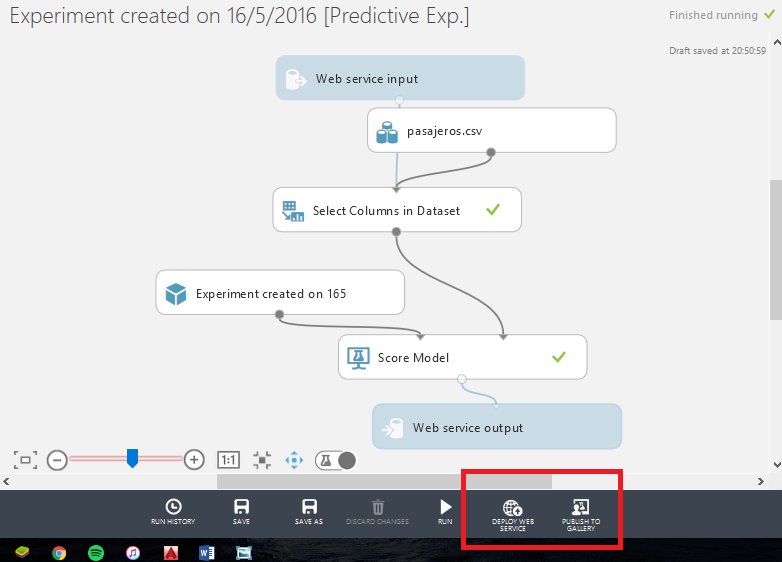
\includegraphics[width=12cm]{10.jpg}
\label{fig:lion}
\end{figure}




\newpage
\section {Conclusiones }

Las Herramientas que nos ofrece hoy en día Microsoft son de vanguardia y más aún están al alcance de todos, por lo que hoy día cualquiera puede ganar y obtener experiencia sobre sus datos, no solo por conocimiento empírico, sino que lo puede hacer de forma automática, utilizando los servicios de Azure y PowerBI, así por tanto debemos compartir este tipo de tecnologías para que muchas personas sean las beneficiadas y se puedan obtener más ingresos. Conocer tu entorno y adelantarte un paso más ahora es más fácil con los servicios de Machinery Learning





\end{document}
